\documentclass[12pt]{article}

\newcommand{\name}{Mike Gao}
\newcommand{\problemset}{ FINAL EXAM }

%\pagestyle{headings}
\usepackage[dvips]{graphics,color}
\usepackage{amsfonts}
\usepackage{amssymb}
\usepackage{amsmath}
\usepackage{latexsym}
\usepackage{enumerate}
\usepackage{graphicx}
\setlength{\parskip}{1pc}
\setlength{\parindent}{0pt}
\setlength{\topmargin}{-3pc}
\setlength{\textheight}{9.5in}
\setlength{\oddsidemargin}{0pc}
\setlength{\evensidemargin}{0pc}
\setlength{\textwidth}{6.5in}
\usepackage{minted}
\newcommand{\answer}[1]{
\newpage
\noindent
\framebox{
	\vbox{
		COMP 557 \hfill {\bf \problemset} \hfill Prof. Paul Kry \\ 
		\name \hfill \today \\
		260915701 \hfill \# #1
	}
}
\bigskip

}
\usepackage{xcolor}

\usemintedstyle{friendly}

\begin{document}

\answer{1}

Given four homogeneous points $p_0 = (9, 12, 6, 1.5)$, $p_1 = (12, 16, 8, 2)$, $p_2 = (9, 12, 6, 1)$, and
$p_3 = (18, 24, 12, 3)$. All of them except one represent the same 3D point. What is that 3D
point, and which of the homogeneous points p 0 , ...p 3 represents a different 3D point?



Common point $(6, 8, 4)$ and $P_2=(9,12,6,1)$ represents a different 3D point.


\answer{2}

Let p A be a point, v A a vector, and n A a normal vector, all expressed in homogeneous
coordinates of reference frame A. Let reference frame B be different from reference frame A. Let the 4x4 matrix M = [x y z c] , where x, y, and z are vectors that specify the axes of frame B in homogeneous coordinates of frame A, and c is a point that specifies the origin of frame B in homogeneous coordinates of frame A. Use the matrix M to write the expressions for computing the point, vector, and normal in coordinates of reference frame B, that is, $p_B$, $v_B$ , and $n_B$ , respectively.

\begin{align*}
p_{uvw} &= [ 0,0, 0, 1] ^{-1} * p_{xyz} \\
p_B &= M^{-1}p_A
\end{align*}

Similarly, $v_B = M^{-1}v_A$

Since Normals are covectors

If dot (t, n) = 0, 
\begin{align*}
M^{-1}t*X &= t^T(M^{-1})^TX = 0 \\
M^{-1}t*X &= I \\
X &= ((M^{-1})^T)^{-1}
\end{align*}

So, $n_B = ((M^{-1})^T)^{-1} n_A $



% PROBLEM 3

\answer{3}

Suppose you are given SpongeBob as a set of points expressed in a 2D coordinate system W. Give a sequence of affine transformations that have the action of rotating the points by 45 degrees counterclockwise while leaving the point at $(x, y) = (4, 3)$ fixed. Use homogeneous representation for your transformations.

$M = T^{-1}RT$ where 
$T= \begin{matrix}
1 & 0 & -4\\
0 & 1 & -3\\
0 & 0 & 1
\end{matrix}$
 and $R= \begin{matrix}
cos(45) & -sin(45) & 0\\
sin(45) & cos(45) & 0\\
0 & 0 & 1
\end{matrix}$

$M = \begin{matrix}
0.707 & -0.707 & 3.293\\
0.707 & 0.707 & -1.950\\
0 & 0 & 1
\end{matrix}$



% PROBLEM 4

\answer{4}
Consider a subdivision curve using the Chaikin scheme averaging mask $(r_{-1}, r_0 , r_1 ) =
(0, 0.5, 0.5)$, which averages the position of a point with its neighbour to the right. In class,
we only saw an example of using the Chaikin scheme to subdivide a closed curve (one
where the end wraps around to the beginning). What is a reasonable special rule to define
for the endpoints of a curve subdivided with the Chaikin scheme?

In the case of an “open shape”, the first and last endpoints shouldn’t be moved. However, in the case of a “closed shape”, we cut all edges on both ends.


% PROBLEM 5

\answer{5}
Whats the difference between even and odd vertices in a subdivision scheme?

Newly created vertices are called odd vertices, while the original vertex are called even vertices.


% PROBLEM 6

\answer{6}

How many real scalar values are necessary to describe the shape of a rational Bezier curve?
Suppose the curve is in d dimensions and the degree of the Bezier is n. What is your answer
when d = 2 and n = 3.

Degree 2 curve needs 3 coefficients so you need 3 points, and in 3D space with rational representation so 4 numbers per data point so $3*4=12$ in total

\answer{7}

\begin{align*} 
    B_{i,n}(t) &=  \binom{n}{i} * t^i (1-t)^{n-i} \\ 
    B_{i,n}(t)'&=  \binom{n}{i}*i*t^{i-1}*(1-t)^{n-i} + (-1)*(n-i)*(1-t)^{n-i-1}\binom{n}{i} t^i \\
    &= \binom{n}{i}(it^{i-1}(1-t)^{n-i} - (n-i)(1-t)^{n-i-1}*t^i)
\end{align*}

Since $B_{i,n}(t)' = 0$
\begin{align*}
    0 &= \binom{n}{i}(it^{i-1}(1-t)^{n-i} - (n-i)(1-t)^{n-i-1}*t^i) \\
    0 &= t^{i-1}(1-t)^{n-i-1}*(i(1-t)-(n-i)*t)
\end{align*}

Therefore
\begin{enumerate}[1]

\item $t = 0$, or
\item $1 - t = 0$ so $t = 1$, or
\item $i(1-t)-(n-i)t = 0$, so $t = \frac{i}{n} $
\end{enumerate}

Now we consider $B_{i,n}(t)'' < 0$

\begin{align*}
    B_{i,n}(t)'' &= \binom{n}{i}((1-t)^{n-i-2}t^{i-2}((i-1)(1-t)(1-nt)-(nt-t-it)*(i-nt)-nt*(1-t)))
\end{align*}

\begin{enumerate}[1]

\item $t = 0$, $B_{i,n}(t)'' = \binom{n}{i} * (i^2-i) \geq 0$
\item $t = 1$, $B_{i,n}(t)'' = \binom{n}{i} * (0) = 0$
\item $t = \frac{i}{n} $, $B_{i,n}(t)'' = \binom{n}{i} * (-i+\frac{i}{n}) \leq 0$
\end{enumerate}

Therefore, local max at $t = \frac{i}{n}$

\answer{8}
Write a parametric equation for the plane that contains the triangle defined by points $A, B, C \in R^3 $.

$p = A + s(B-A) + t(C-A)$

% PROBLEM 9

\answer{9}
Write an implicit equation for the plane that contains the triangle defined by points $A, B, C \in R^3 $.

\begin{center}
$n = cross(B-A, C-A)$

$n * (p-A) = 0$

$n.x (x-A.x) + n.y (y-A.y) + n.z (z-A.z) = 0$

$n.x*x+n.y*y+n.z*z = n.x*A.x + n.y*A.y + n.z*A.z$
\end{center}

% PROBLEM 10
\answer{10}
List the most important advantages and disadvantages of triangles and quadrilaterals.

Pro for triangles / Con for Quadrilaterals
\begin{enumerate}[(1)]
\item Always planar
\item Never self intersect
\item Irreducible to simpler polygons
\item Can use barycentric coordinates - allows you to easily assign a property, such as color, at each vertex and smoothly interpolate the value across a triangle.
\end{enumerate}

Con for triangles / Pro for Quadrilaterals

For stuff like city architecture, triangle increases storage requirement without increasing model resolution.


% PROBLEM 11
\answer{11}
Describe and sketch a mesh which is an orientable manifold with one boundary and genus one. Note you do not need to draw the mesh showing all the faces. You just need to draw enough to illustrate your answer.

\begin{center}
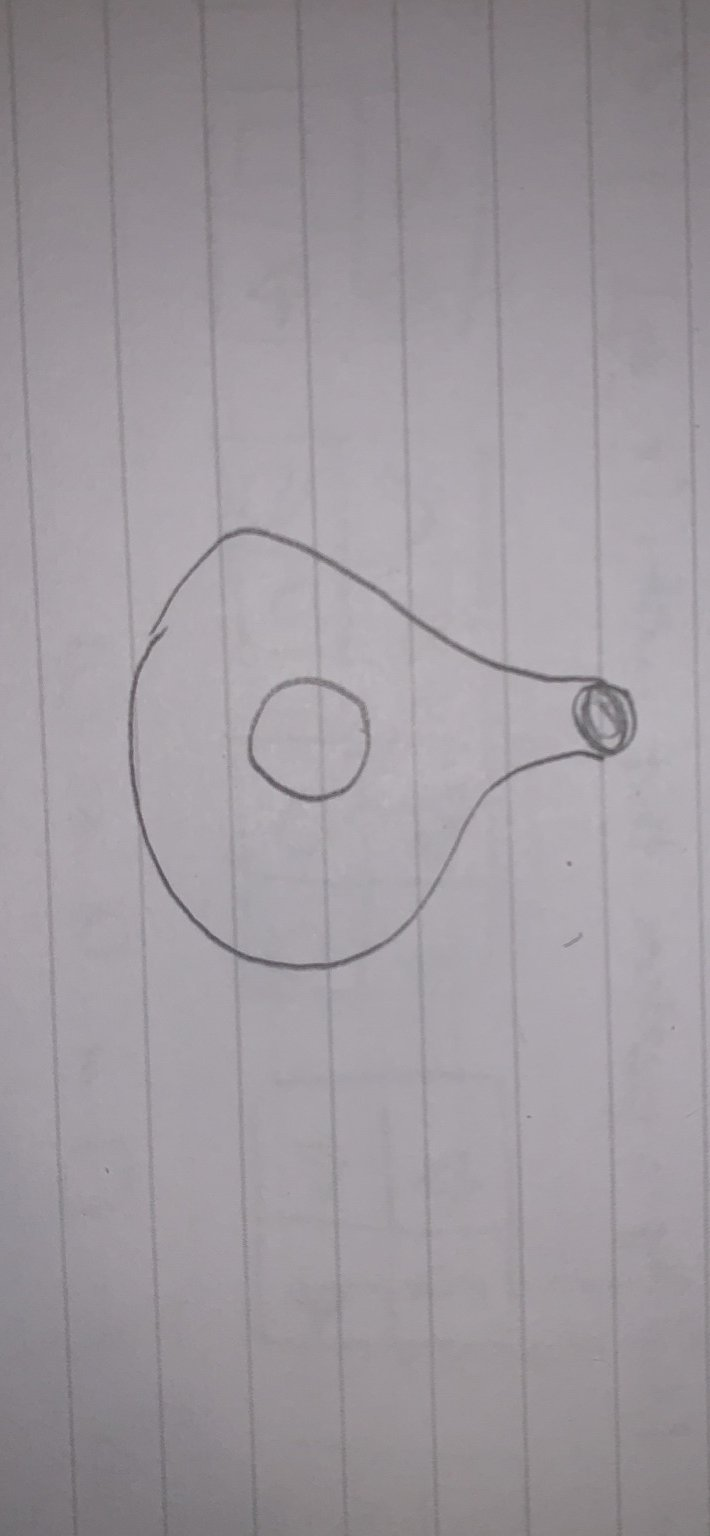
\includegraphics[width=3cm, height=7cm]{torus.jpeg}
\end{center}

Torus with a hole.

% PROBLEM 12
\answer{12}
Write pseudocode for method CollapseEdge( HalfEdge e, Vertex v ), which performs an edge collapse on a half edge data structure. The method takes as parameter a half
edge e specifying the edge to collapse, and a new vertex v with the new position for the
collapsed edge vertices. Assume the mesh is a watertight manifold (i.e., no boundaries).
You may also assume that the two faces involved will be removed from the face list by the
caller. Draw a diagram with labels on the mesh around the edge being collapsed to help
explain variables in your code.

Assuming you only have triangular faces

\begin{center}
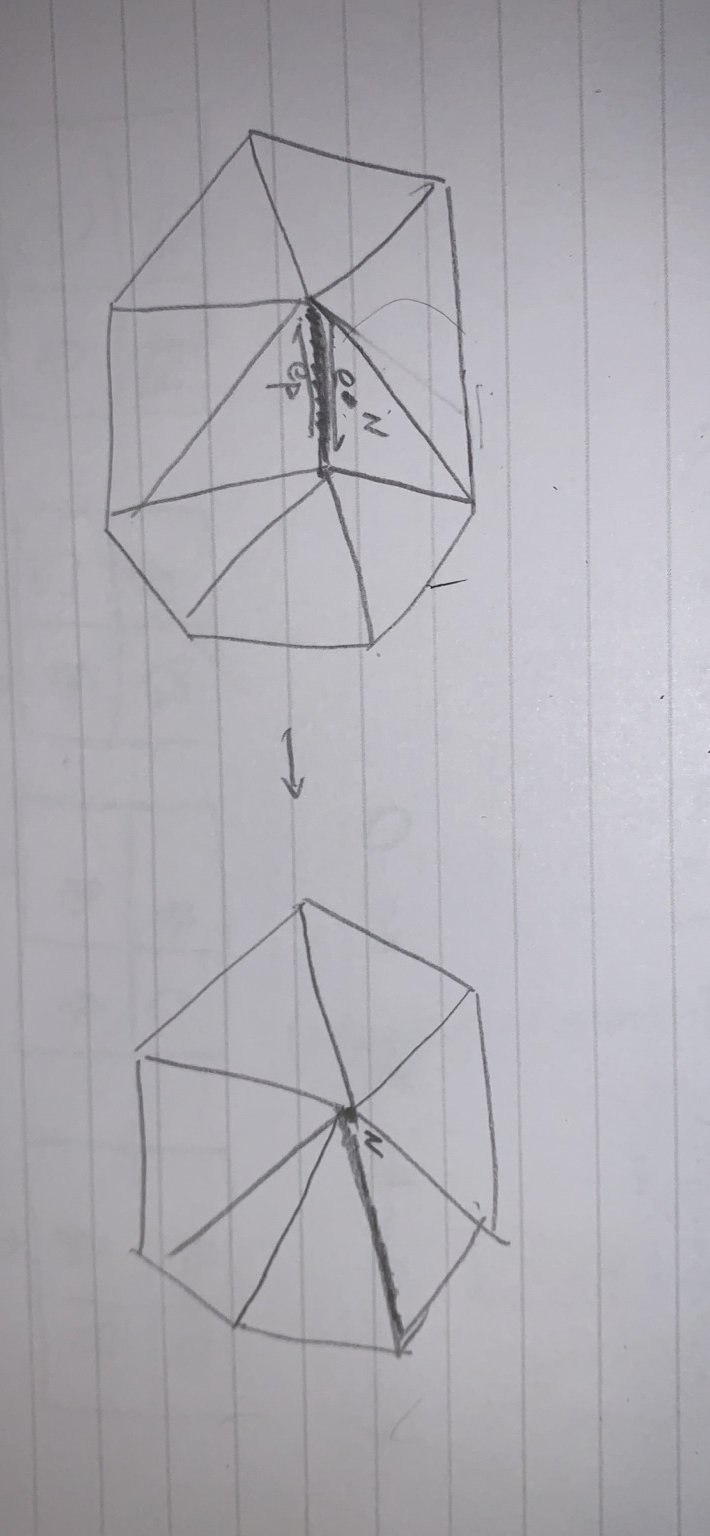
\includegraphics[angle=90,width=15cm, height=7cm]{edge_collapse.jpeg}
\end{center}

\newpage

\begin{minted}{glsl}
CollapseEdge(HalfEdge e, Vertex v){
    HalfEdge e_pair = e-> pair
	if (e -> vertex == v) {
		swap(e, e_pair)
	}
	// edge to remove pair
	Vertex e_vertex = e -> vertex
	Vertex ep_vertex = e_pair -> vertex
	// get faces that share the endpoint of this edge
	// get faces that border this edge
	HalfEdge e_next = e -> next
	HalfEdge e_prev = e -> next -> next
	HalfEdge e_next_pair = e_next -> pair
	HalfEdge e_prev_pair = e_prev -> pair
	HalfEdge ep_next = e_pair -> next
	HalfEdge ep_prev = e_pair -> next -> next
	HalfEdge ep_next_pair = ep_next -> pair
	HalfEdge ep_prev_pair = ep_prev -> pair
	// we need to fix surrounding edges that points to vertex that’s removed
	HalfEdge cur = e_vertex -> edge -> pair
	HalfEdge first = e_vertex -> edge -> pair
	// reassign all vertices from removed one to next
	do {
		cur -> vertex = ep_vertex
		cur = cur-> next -> pair
	} while (cur != first)
	if (ep_vertex -> edge == e || ep_vertex -> edge = e_next) {
		ep_vertex -> edge = ep_prev ->pair
	}
	e_next_pair -> pair = e_prev_pair
	e_prev_pair -> pair = e_next_pair
	ep_next_pair -> pair = ep_prev_pair
	ep_prev_pair -> pair = ep_next_pair
	erase(e_vertex, ep_next, ep_prev, e_next, e_prev, e, e_pair)
}

\end{minted}

\answer{13}

Suppose you are rendering an image to a HD screen, 1920 by 1080 pixels, and have a vertical FOV of 27 degrees. You have have an eye point at 10 units on the positive z axis
and a look at the point set to the origin, and y axis as the up direction. The scene consists of a 1 unit by 1 unit square, centered at the origin or the world, with normal in the z direction.
The square has a texture stored in a 512x512 image. Does this scenario need a minification
filter or a magnification filter? Show your work to explain your answer.

\begin{center}

$512 * 512  = 262144$ texels / unit square

$1920 * 1080 = 2073600$ pixels

Fovy = 27 deg, $tan(\frac{27}{2}) = 0.24008 = h / (2 * depth)$

$h = 4.8016$

$4.8016 *1920 / 1080 = 8.5362$

Total area viewed at depth 10: $4.8016*8.5362 = 40.9874$

$2073600/40.9874=50591.157$ pixels / unit

texel/pixel $> 1$ thus need minification filter
\end{center}


\answer{14}
Suppose you must compute texture coordinates for a leg of an animated character. In its
local coordinates, suppose it is centered at the origin and the length of the leg is oriented
in the z axis. Write pseudocode to compute a cylinder mapping, that is, for every vertex v
compute a texture coordinate in the interval [0,1] using a cylinder mapping.

\begin{minted}{glsl}
CylindricalMap(vertex vert) {
	// compute the azimuthal angle
	theta = arctan2(vert.x, vert.y)
	// radians to -0.5< u <= 0.5
	u = theta / 2 / pi
	// convert it to correct scale 
	// flip so u increases with theta counter clockwise
	u = 1 - u - 0.5
	// let v go from 0 to 1 between every unit of vert.z
	v = vert.z mod 1
	return (u,v)
}
\end{minted}

\answer{15}
What kind of projection would you use to create a shadow map texture for a directional light

We use orthographic projection

\answer{16}

In the following diagram, the one eyed monster has designed a matrix so that a glowing
luminous coloured disk has the same appearance in real life as it does when displayed on
the monitor. Suppose that the camera is special in that it records a discretized vector s for
spectral power density at each pixel. Assume that the monster has cone receptors on his
retina identical to those of a human. Describe how this is possible (to design such a matrix)
and under what conditions the colours can actually be made to match.

\begin{enumerate}
    \item When monster directly look at the disk\\
        Transform: real spectrum  $ \rightarrow$ visual response space, so only need to apply $M_{SML}$
    \item When monster is looking at the display\\
        Transform: Camera records the discretized vector s for each pixel's spectral power density $\rightarrow$ RGB $\rightarrow$ monitor produces spectral power density at each pixel $\rightarrow$ visual response space
\end{enumerate}

We first define a matrix that maps vectors in the discrete SPD space from the output of the camera $s$ to the response function of the monitor $V=M_{SML} s$

We then define a matrix that maps the RGB color of the monitor to the visual spectrum $s_v=M_{RGB}C$

The color we see at the display $V = M_{SML} M_{RGB} C$

We then know the color matching matrix is $C = (M_{SML} M_{RGB})^{-1} M_{SML} s$

Color matching relies on the monitor to be able to display the color at the specific color value its given. If it is a color that cannot be displayed by the monitor (for example, if the monitor fail to display some color within the visual spectrum because that color is outside of the monitor's color gamut, color matching attemp will fail).

\end{document}



